%! Author = adnansiddiquei
%! Date = 08/03/2024

\section{Development, Experimentation, Profiling and Optimisation}\label{sec:development}
    This section discusses the experimentation and profiling of the different methods discussed in the previous
    section (Section \eqref{sec:prototyping}).
    Most of the experimentation was done on a Macbook M1 Pro (10 cores; 16GB RAM; 128 KB of L1 data cache; 192 KB of L1
    instruction cache; 64 Byte cache line size; 4 MB of L2 cache), which is why the number of OpenMP threads for local
    experimentation was limited to 10.
    \subsection{Profiling the Convolution Methods}\label{subsec:prof-conv}
    \begin{figure}[htb]
    \centering
    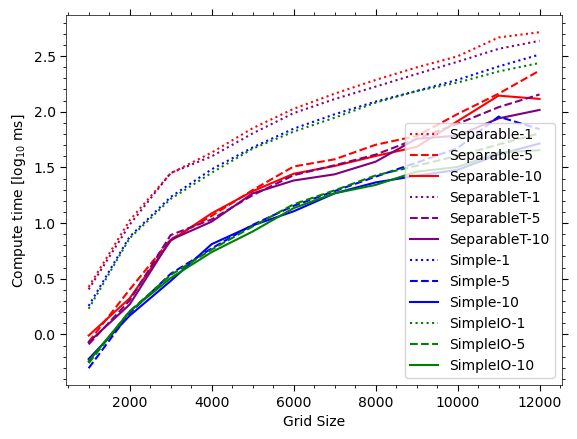
\includegraphics[width=0.75\textwidth]{./figures/convolutions}
    \caption{A figure showing the compute time for 4 of the convolution methods for counting neighbours.
        The colour of the line indicates the method used, and the line style (dotted, dashed, solid) indicates the number
        OpenMP threads used (1, 5 and 10 respectively).
        Only 1 MPI rank was used.
        The x-axis shows the size of one dimension of the square grid.
        The Simple and Separable methods are as described in \eqref{subsec:domain-decomp} and the SimpleIO method is
        as described in \eqref{subsec:hiding-comms})
        The SeparableT method is the Separable method done in 2 horizontal passes with a transpose in between, except
        the time on the graph is just the compute time to repeast the first horizontal pass twice (i.e, it is the time
        for the actual SeparableT method minus the tranpose compute time).
        This was done for simplicity, to assess whether a tranpose operation needed coding.
        The compute time is averaged over 3 runs.}
    \label{fig:convolutions}
    \end{figure}

    Fig.\eqref{fig:convolutions} shows the compute time across 4 different convolution methods for counting neighbours
    and how they scale with \inlinecode{grid_size} and \inlinecode{OMP_NUM_THREADS}.
    The first observation is that both the simple methods are faster than both of the separable methods, which is
    at face value, unexpected.
    Furthermore, there is a negligible difference in speed between the Simple and SimpleIO method which is a positive
    outcome which means the SimpleIO method is a good candidate for hiding communication overheads, as the vast majority
    of the computation can be done while waiting for the communication to complete.
    It is worth noting that all of these methods show diminishing returns as the number of OMP threads increases.
    \begin{figure}[htb]
    \centering
    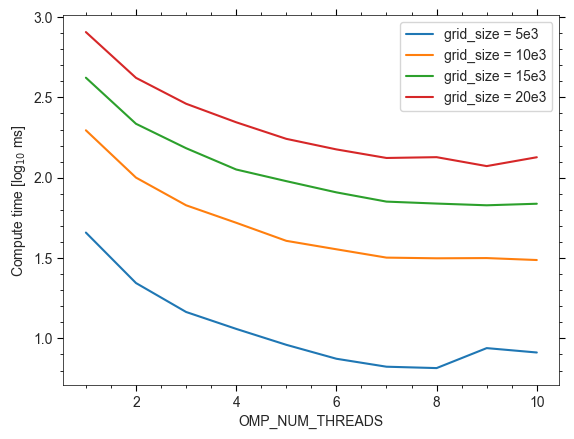
\includegraphics[width=0.75\textwidth]{./figures/simpleio}
    \caption{A figure showing how the compute time varies for the SimpleIO method as the number of OMP threads is changed.
    1 MPI rank was used, and compute time is averaged over 3 runs.}
    \label{fig:simpleio}
    \end{figure}

    Fig.\eqref{fig:simpleio} shows that as the number of OMP threads increases, the compute time decreases, but with
    diminishing returns.
    The jump from 1 to 2 threads yields a 2x increase but jumps following this do not yield speed increases in the same
    proportion.
    At about 8 threads, the returns on increasing the number of threads become negligible, which is useful information
    for optimising the MPI rank to OMP thread ratio.

    The analysis thus far has yielded the following conclusions: the SimpleIO method is a good candidate for counting
    neighbours and hiding MPI communication overheads; and 8 may be a reasonable cap on the optimal number of OMP threads.

    \subsection{Profiling the Update Methods}\label{subsec:prof-trans}
        \begin{figure}[htb]
    \centering
    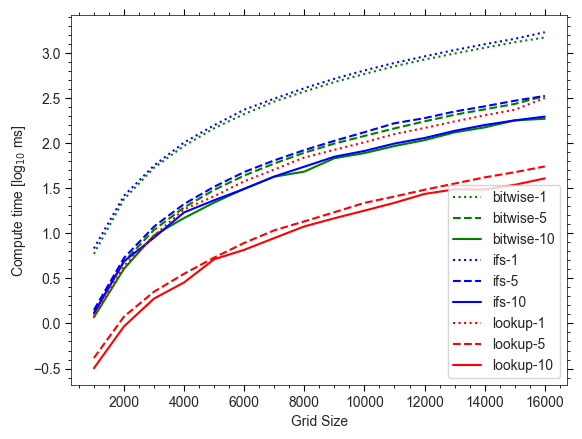
\includegraphics[width=0.75\textwidth]{./figures/transitions}
    \caption{A figure showing the compute time for the 3 the update methods discussed in Section \eqref{subsec:update-grid}.
        The colour of the line indicates the method used, and the line style (dotted, dashed, solid) indicates the number
        OpenMP threads used (1, 5 and 10 respectively).
        Only 1 MPI rank was used.
        The compute time is averaged over 3 runs.}
    \label{fig:transitions}
    \end{figure}

    Fig.\eqref{fig:transitions} explores the update methods discussed in Section \eqref{subsec:update-grid}, with a
    clear conclusion that the lookup method is the fastest, and as expected, the \inlinecode{if} method is the slowest.
    This makes sense, due to the (effectively) random nature of the simulation, the CPU will have little success
    in branch predictions, contributing to the slowness of the \inlinecode{if} method down.
    The frequent lookup in an 18-length array is relatively inexpensive compared to frequent branching.




